\subsection{Full-core TAP MSR Serpent model}


\begin{frame}
\frametitle{TAP concept design}

\begin{textblock*}{12.5cm}(0.2cm,1.7cm) % {block width} (coords)
	
	\begin{columns}
		\column[t]{6cm}
			\vspace{+5mm}
	%%%%%%%%%%%%%%%%%%%%%%%%%%%%%%%%%%%%%%%%
	\begin{table}[h!]
		\fontsize{7}{10}\selectfont
	\caption{Summary of principal data for the \gls{TAP} \gls{MSR} 
		\cite{transatomic_power_corporation_technical_2016, 
			betzler_assessment_2017}. }
		\vspace{-2mm}
	\begin{tabularx}{\textwidth}{ X  X }
		\hline
		Thermal power				           		& 1250 MW$_{th}  $       
		\\ 
		Electric power		                		& 520 MW$_e  $ 			 
		\\ 
		Gross thermal efficiency        			& 44\%     				 
		\\  
		Outlet temperature							& 620$^{\circ}$C         
		\\ 
		Fuel salt components                   & LiF-UF$_4$				 \\  
		Fuel salt composition                  & 72.5-27.5 mole\%			 
		\\  
		Startup fissile material                     & 5\% 
		$^{235}$U          	 \\
		Moderator                              & Zirconium Hydride 
		(ZrH$_{1.66}$) rods (with silicon carbide cladding) \\
		Neutron spectrum						& 
		thermal/epithermal                 \\
		\hline
	\end{tabularx}
	\label{tab:tap_tab}
	\end{table}
	%%%%%%%%%%%%%%%%%%%%%%%%%%%%%%%%%%%%%%%%%%%%%%%%
		
		\column[t]{5.5cm}
			\hspace{-9mm}
		\begin{figure}      
			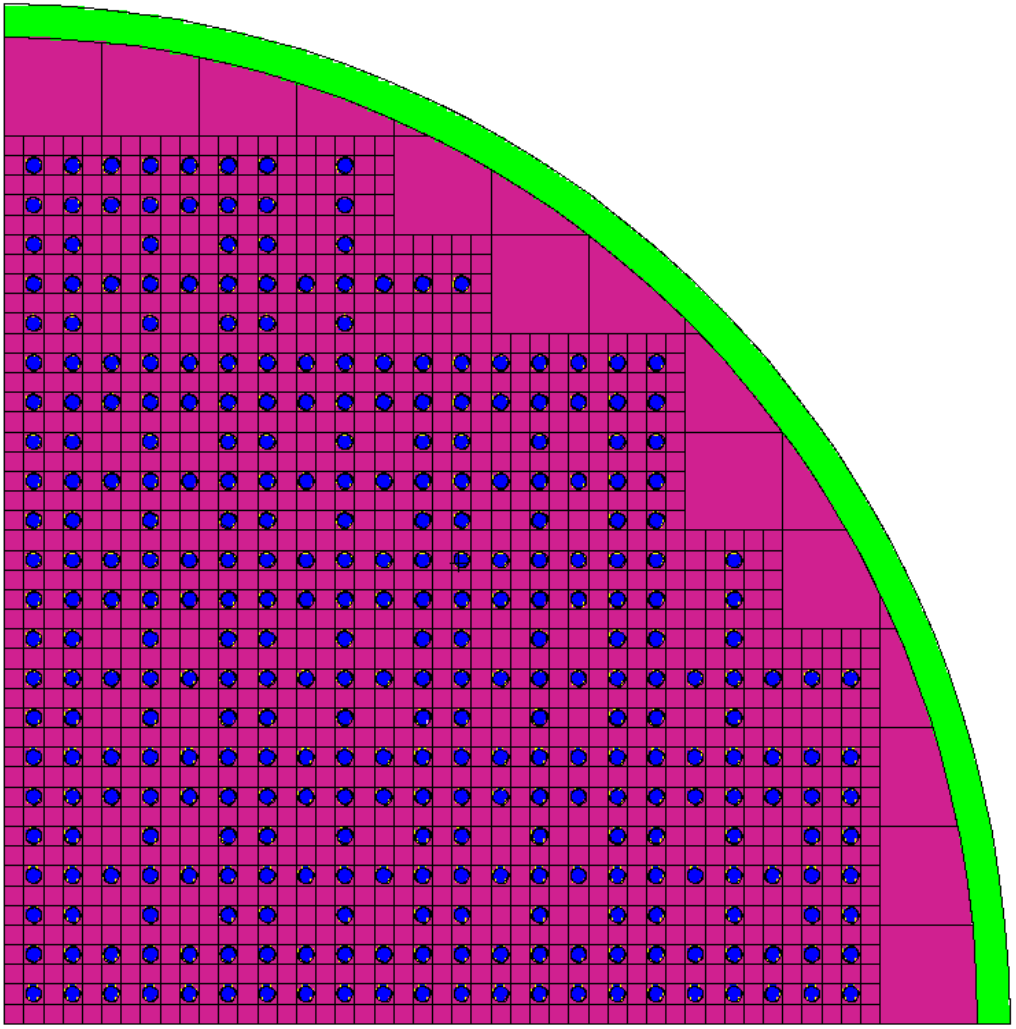
\includegraphics[height=1.03\textwidth]{./images/tap_core_ornl.png}
			\caption{The \gls{TAP} \gls{MSR} schematic core view showing 
			moderator rods \cite{betzler_assessment_2017}.}
		\end{figure}
	\end{columns}
	
\end{textblock*}

\end{frame}


\begin{frame}
\frametitle{\gls{TAP} concept full-core high-fidelity Serpent model}
\begin{textblock*}{12.25cm}(0.25cm,1.8cm) % {block width} (coords)
	\begin{figure}[htp!] % replace 't' with 'b' to 
		
\includegraphics[width=\textwidth]{./images/tap_model.png}
		\caption{An $XY$ (left) and $XZ$ (right) section of the \gls{TAP} 
		model. The violet color represents zirconium hydride, the yellow 
		represents fuel salt \cite{rykhlevskii_milestone_2019}.}
	\end{figure}
\end{textblock*}
\end{frame}


\subsection{Load Following transient}

\begin{frame}
\frametitle{Postulated worst-case load following scenario}
\vspace{-6mm}
\begin{columns}
	\column[t]{5.5cm}
	\begin{figure}[t]
		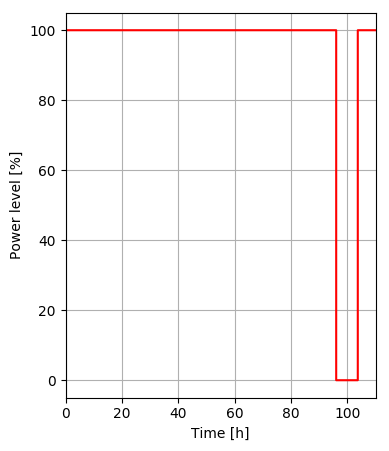
\includegraphics[width=\linewidth]{./images/power_load_curve.png}
		\vspace{-6mm}
		\caption{Assumed load-following power variation.}
	\end{figure}
	
	\column[t]{6cm}
	\begin{block}{Assumed worst-case power variation}
		\begin{enumerate}             
			\item Startup with fresh fuel and operating on 100\% power
			level for \textbf{96 hrs} to reach $^{135}$Xe/$^{135}$I balance
			\item \textbf{Instantaneous power} level drop from 100\% to 0\%
			\item Shutdown state for \textbf{7.66 hrs} to reach the 
			$^{135}$Xe peak
			\item Instantaneous power boost from 0 to 100\%, then operation 
			on 100\% for \textbf{16 hrs}
		\end{enumerate}
	\end{block}
			\vspace{-2mm}
	\begin{block}{Simplifying assumptions}
		\begin{itemize}
			\item All control rods are fully withdrawn
			\item Online reprocessing system is \textbf{disabled}
			\item 15-min depletion steps in the transient
			\item Delayed
neutron precursor drift ignored
		\end{itemize}

	\end{block}
\end{columns}
\end{frame}